\documentclass[11pt,a4paper]{article}

\usepackage{amsmath,amssymb,amsthm}
\usepackage[ruled,vlined]{algorithm2e}
\usepackage{booktabs}
\usepackage[margin=2.5cm]{geometry}
\usepackage{hyperref}
\usepackage{tikz}
\usetikzlibrary{arrows.meta,positioning}

\hypersetup{colorlinks=false}

\title{MP4-to-GIF Converter:\\Mathematical Foundations and Algorithmic Analysis}
\author{}
\date{\today}

\begin{document}
\maketitle
\tableofcontents
\newpage

%============================================================================
\section{Color Space Quantization}
%============================================================================

\subsection{Histogram Construction (Hist3D)}

RGB space is quantized to a $33 \times 33 \times 33$ lattice.
Each channel is reduced to 5-bit resolution with a $+1$ offset to reserve
index 0 for boundary padding:
\begin{equation}
  b(r,g,b) = \left(\lfloor r/8 \rfloor + 1,\;
               \lfloor g/8 \rfloor + 1,\;
               \lfloor b/8 \rfloor + 1\right)
             \in [1,32]^3
\end{equation}

Linear index: $i = r \cdot 33^2 + g \cdot 33 + b$.

Five moment arrays are accumulated per bin~$i$:
\begin{align}
  w_i     &= \sum_{p \in \mathrm{bin}_i} 1
             & &\text{(pixel count)} \\
  m^R_i   &= \sum_{p} R_p,\quad
  m^G_i    = \sum_{p} G_p,\quad
  m^B_i    = \sum_{p} B_p
             & &\text{(first moments)} \\
  m^2_i   &= \sum_{p} (R_p^2 + G_p^2 + B_p^2)
             & &\text{(second moment)}
\end{align}

Total memory: $5 \times 33^3 \times 4 \approx 700\,\text{KB}$
(four \texttt{int32\_t} arrays + one \texttt{float} array).

%----------------------------------------------------------------------------
\subsection{Cumulative 3D Prefix Sums}

Raw histograms are converted to cumulative form via Wu's M3d pattern.
For each moment array $A$, the cumulative value at $(r,g,b)$ stores the
sum over all bins $[0,r] \times [0,g] \times [0,b]$:
\begin{equation}
  A[r,g,b] = \sum_{r'=0}^{r} \sum_{g'=0}^{g} \sum_{b'=0}^{b}
              A_{\mathrm{raw}}[r',g',b']
\end{equation}

Computed in $O(33^3)$ using running line and area accumulators.
For each fixed $r$, the algorithm maintains:
\begin{align}
  \texttt{line}[b] &= \sum_{b'=1}^{b} A_{\mathrm{raw}}[r,g,b'] \\
  \texttt{area}[b] &\mathrel{+}= \texttt{line}[b] \\
  A[r,g,b] &= A[r-1,g,b] + \texttt{area}[b]
\end{align}

After this transformation, any box query uses 8-corner inclusion-exclusion.
For box $B = [r_0, r_1] \times [g_0, g_1] \times [b_0, b_1]$:
\begin{equation}
  \mathrm{Vol}(B, A) = \sum_{\mathbf{s} \in \{0,1\}^3}
    (-1)^{|\mathbf{s}|} \; A\!\left[\, r_{s_0},\, g_{s_1},\, b_{s_2} \,\right]
\end{equation}

%----------------------------------------------------------------------------
\subsection{Wu's Optimal Quantization}

The variance of a box $B$ is:
\begin{equation}
  \hat{\sigma}^2(B) = M_2(B)
    - \frac{M_R(B)^2 + M_G(B)^2 + M_B(B)^2}{w(B)}
\end{equation}

where $w(B) = \mathrm{Vol}(B, \mathbf{w})$,
$M_c(B) = \mathrm{Vol}(B, \mathbf{m}^c)$ for $c \in \{R,G,B\}$,
$M_2(B) = \mathrm{Vol}(B, \mathbf{m}^2)$.

\medskip
\noindent\textbf{Greedy Splitting:}
\begin{enumerate}
  \item Initialize $B_0 = [0,32]^3$, compute $\hat{\sigma}^2(B_0)$.
  \item Select $B^* = \arg\max_i \hat{\sigma}^2(B_i)$.
  \item For each axis $a \in \{R, G, B\}$, find optimal cut:
    \begin{equation}
      c^*_a = \arg\max_{c}
        \left[
          \frac{\sum_c M_c^2}{w}\bigg|_{\mathrm{bottom}(c)}
        + \frac{\sum_c M_c^2}{w}\bigg|_{\mathrm{top}(c)}
        \right]
    \end{equation}
  \item Split along axis with maximum reduction, recompute variances.
\end{enumerate}

Palette extraction via weighted centroid per box:
\begin{equation}
  P_i = \left(
    \frac{M_R(B_i)}{w(B_i)},\;
    \frac{M_G(B_i)}{w(B_i)},\;
    \frac{M_B(B_i)}{w(B_i)}
  \right)
\end{equation}

%----------------------------------------------------------------------------
\subsection{Median-Cut Quantization}

Priority queue ordered by pixel count $|B|$. Splitting rule: longest axis.
\begin{equation}
  a^* = \arg\max_{c \in \{R,G,B\}} (c_{\max} - c_{\min})
\end{equation}

Split at population median: find position $s$ such that
$\sum_{i=a_{\min}}^{s} n_i \geq |B|/2$.

%----------------------------------------------------------------------------
\subsection{Nearest-Color Cache}

A $32^3$ cache indexed by 5-bit quantized RGB.
Distance metric:
\begin{equation}
  d(p, q) = (R_p - R_q)^2 + (G_p - G_q)^2 + (B_p - B_q)^2
\end{equation}

\noindent\textbf{AVX2 precomputation:} palette colors are deinterleaved into
SoA layout (aligned \texttt{int16\_t} arrays $\mathbf{r}[256]$,
$\mathbf{g}[256]$, $\mathbf{b}[256]$). For each of $32^3$ cache entries,
16 palette entries are processed per SIMD iteration:
\begin{align}
  \mathbf{d}_r &= \mathrm{vpsub}(\mathbf{q}_r, \mathbf{p}_r) \\
  d_{rg} &= \mathrm{vpmaddwd}([\mathbf{d}_r, \mathbf{d}_g],
                               [\mathbf{d}_r, \mathbf{d}_g]) \\
  d_{\mathrm{total}} &= d_{rg} + \mathrm{vpmaddwd}([\mathbf{d}_b, \mathbf{0}],
                                                     [\mathbf{d}_b, \mathbf{0}])
\end{align}

Runtime dispatch via \texttt{\_\_builtin\_cpu\_supports("avx2")}.
Cache is \texttt{thread\_local}, 32\,KB. Amortized $O(1)$ per pixel.

%============================================================================
\section{Dithering}
%============================================================================

\subsection{Floyd-Steinberg Error Diffusion}

Error $\mathbf{e} = \mathbf{c}_{\mathrm{in}} - \mathbf{c}_{\mathrm{palette}}$
diffused via kernel (serpentine scan):
\begin{equation}
  \frac{1}{16}\begin{bmatrix}
    \cdot & \cdot & \cdot \\
    \cdot &   *   &   7   \\
      3   &   5   &   1
  \end{bmatrix}
\end{equation}

Implementation uses error-only two-row ring buffer:
$2 \times (W+2) \times 3$ \texttt{int16\_t} values. No RGB copy,
no bounds checks (padding absorbs boundary errors).
Nearest-color lookup inlined as direct cache array access:
\texttt{inv\_cache[r>>3][g>>3][b>>3]}.

%----------------------------------------------------------------------------
\subsection{Bayer Ordered Dithering}

Threshold application with spread $s = 48$:
\begin{equation}
  \mathbf{c}'(x,y) = \mathrm{clamp}\!\left(
    \mathbf{c}(x,y) + \frac{(M_8[y \bmod 8][x \bmod 8] - 32) \cdot s}{64},\;
    0,\; 255
  \right)
\end{equation}

No inter-pixel dependencies (fully parallelizable).

%============================================================================
\section{GIF Encoding}
%============================================================================

\subsection{LZW Compression}

Hash-table string matching with 12-bit codes.
Table: 8192 entries (power-of-2, open addressing with linear probing).
Key: $(\mathrm{prefix} \ll 8) \mathbin{|} \mathrm{suffix}$.
Hash: $((\mathrm{key} \gg 12) \oplus \mathrm{key}) \mathbin{\&} 8191$.

\medskip
\noindent Bit packing via 64-bit accumulator:
\begin{equation}
  \mathrm{acc} \mathrel{|}= (\mathrm{code} \ll \mathrm{bits}), \quad
  \text{while } \mathrm{bits} \geq 8: \text{emit byte, shift right 8}
\end{equation}

Output staged into 32\,KB buffer, flushed as GIF sub-blocks
(max 255 bytes each). Table reset on overflow ($\mathrm{code} > 4095$)
via clear code emission.

%----------------------------------------------------------------------------
\subsection{GIF89a Binary Writer}

Direct binary output (no giflib dependency):
\begin{center}
\begin{tabular}{@{}lrl@{}}
\toprule
  Block & Bytes & Content \\
\midrule
  Header & 6 & \texttt{GIF89a} \\
  Logical Screen Descriptor & 7 & $W$, $H$, packed flags \\
  Global Color Table & 768 & $256 \times$ RGB \\
  NETSCAPE 2.0 Extension & 19 & Infinite loop \\
  Per-frame GCE & 8 & Delay (cs), disposal \\
  Per-frame Image Descriptor & 10 & Position, dimensions \\
  Per-frame LZW Data & var & Sub-block stream \\
  Trailer & 1 & \texttt{0x3B} \\
\bottomrule
\end{tabular}
\end{center}

\subsection{Timing Model}

Drift-free microsecond-to-centisecond conversion:
\begin{align}
  \mathrm{acc}_{\mu\mathrm{s}} &\mathrel{+}= \Delta t_{\mu\mathrm{s}} \\
  \mathrm{delay}_{\mathrm{cs}} &= \left\lfloor
    \frac{\mathrm{acc}_{\mu\mathrm{s}} + 5000}{10000}
  \right\rfloor - \mathrm{emitted}_{\mathrm{cs}}, \quad
  \mathrm{delay} \geq 2
\end{align}

Minimum 2\,cs enforced (browsers interpret $< 2$\,cs as 100\,ms).

%============================================================================
\section{Pipeline Architecture}
%============================================================================

Single-decode pipeline with frame caching:

\begin{center}
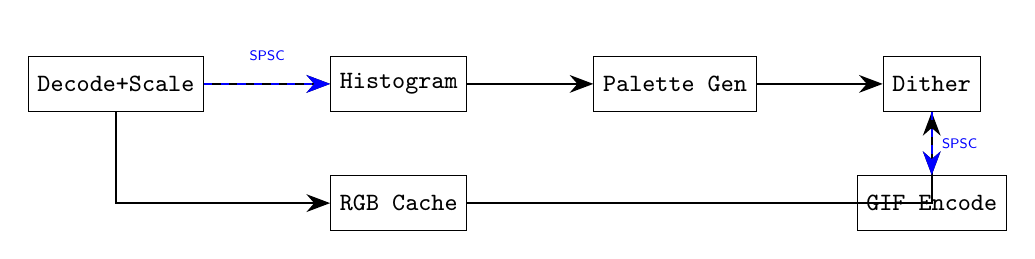
\begin{tikzpicture}[
  node distance=0.8cm and 1.6cm,
  every node/.style={
    draw, rectangle, minimum height=0.7cm,
    font=\small\ttfamily
  },
  arr/.style={-{Stealth[length=3mm]}, thick},
  par/.style={-{Stealth[length=3mm]}, thick, dashed, blue}
]
  \node (dec) {Decode+Scale};
  \node (hist) [right=of dec] {Histogram};
  \node (cache) [below=of hist] {RGB Cache};
  \node (pal) [right=of hist] {Palette Gen};
  \node (dith) [right=of pal] {Dither};
  \node (gif) [below=of dith] {GIF Encode};

  \draw[arr] (dec) -- (hist);
  \draw[arr] (dec) |- (cache);
  \draw[arr] (hist) -- (pal);
  \draw[arr] (cache) -| (dith);
  \draw[arr] (pal) -- (dith);
  \draw[arr] (dith) -- (gif);

  \draw[par] (dec) -- node[draw=none,above,font=\tiny\sffamily,blue] {SPSC} (hist);
  \draw[par] (dith) -- node[draw=none,right,font=\tiny\sffamily,blue] {SPSC} (gif);
\end{tikzpicture}
\end{center}

\noindent\textbf{Key insight:} video decoded once. RGB frames cached in memory
during histogram accumulation, then consumed directly by dither stage.
Eliminates redundant seek + decode + scale pass.

\subsection{Threading Model}

Two SPSC lock-free ring buffers (\texttt{alignas(64)} atomics,
power-of-2 slots):

\begin{enumerate}
  \item \textbf{Decode $\parallel$ Histogram:} producer decodes + scales
        frames, consumer accumulates histogram and stores RGB data.
  \item \textbf{Dither $\parallel$ GIF Encode:} main thread dithers cached
        frames, pushes indexed frames to encoder thread via ring buffer.
\end{enumerate}

\noindent Memory trade-off: $F \times W \times H \times 3$ bytes cached.
For 283 frames at 1080p $\approx 1.7\,$GB. Freed progressively after
each frame is dithered (\texttt{swap} with empty vector).

\subsection{Frame Skipping}

Minimum PTS interval for target FPS:
\begin{equation}
  \mathrm{pts\_step} = \left\lfloor
    \frac{1}{\mathrm{fps}_{\mathrm{target}} \times \mathrm{tb\_seconds}}
  \right\rfloor
\end{equation}

Frame accepted iff $\mathrm{pts} - \mathrm{pts}_{\mathrm{last}} \geq
\mathrm{pts\_step}$.

%============================================================================
\section{RAII Resource Management}
%============================================================================

Template deleters for FFmpeg types:
\begin{center}
\begin{tabular}{@{}lll@{}}
\toprule
  Alias & FFmpeg Type & Deleter \\
\midrule
  \texttt{FormatCtx} & \texttt{AVFormatContext} &
    $\mathrm{Deleterp}\langle\texttt{avformat\_close\_input}\rangle$ \\
  \texttt{CodecCtx} & \texttt{AVCodecContext} &
    $\mathrm{Deleterp}\langle\texttt{avcodec\_free\_context}\rangle$ \\
  \texttt{Frame} & \texttt{AVFrame} &
    $\mathrm{Deleterp}\langle\texttt{av\_frame\_free}\rangle$ \\
  \texttt{Packet} & \texttt{AVPacket} &
    $\mathrm{Deleterp}\langle\texttt{av\_packet\_free}\rangle$ \\
  \texttt{SwsCtx} & \texttt{SwsContext} &
    $\mathrm{Deleter}\langle\texttt{sws\_freeContext}\rangle$ \\
\bottomrule
\end{tabular}
\end{center}

%============================================================================
\section{Complexity Summary}
%============================================================================

\begin{center}
\begin{tabular}{@{}llll@{}}
\toprule
  Algorithm & Time & Space & Notes \\
\midrule
  Histogram build &
    $O(N)$ & $O(33^3)$ &
    $N$ = total pixels \\
  Prefix sums &
    $O(33^3)$ & in-place &
    Single pass \\
  Wu quantization &
    $O(N + K \cdot 33^3)$ & $O(33^3)$ &
    Dominated by histogram \\
  Median-cut &
    $O(K \cdot 33^3)$ & $O(K)$ &
    PQ + recount \\
  Nearest-color cache &
    $O(32^3 \cdot K)$ init & $O(32^3)$ &
    AVX2: 16 entries/iter \\
  Floyd-Steinberg &
    $O(WH)$/frame & $O(W)$ &
    2-row error ring \\
  Bayer &
    $O(WH)$/frame & $O(1)$ &
    No state \\
  LZW compress &
    $O(WH)$/frame & $O(8192)$ &
    Hash table \\
  Full pipeline &
    $O(F \cdot WH)$ & $O(F \cdot WH)$ &
    Frame cache \\
\bottomrule
\end{tabular}
\end{center}

\end{document}
